\documentclass{article}
\usepackage[T1]{fontenc}
\usepackage[utf8]{inputenc}
\usepackage[italian]{babel}
\usepackage{amssymb}

%%%%%%%%%%%%%%%%%%%%%%%%%%%%%%%%%%%%%%%%%%%%%%%%%%%%%%%%%%%%%%%%%%%%%%%%%%%%%%%%%%%%%%%%%%%%
%%%%%%%%%%%%%%%%%%%%%%%%%%%%%%%%%%%%%%%%%%%%%%%%%%%%%%%%%%%%%%%%%%%%%%%%%%%%%%%%%%%%%%%%%%%%
%%%%%%%%%%%%%%%%%%%%%%%%%%%%%%%%%%%%%%%%%%%%%%%%%%%%%%%%%%%%%%%%%%%%%%%%%%%%%%%%%%%%%%%%%%%%

\usepackage{fontawesome5}
\usepackage{robustcommand}
\usepackage{hyperref}
\usepackage{framed}
\usepackage{minted} % loads fancyvrb
\usepackage{float}

% https://tex.stackexchange.com/questions/28205/remove-colon-from-table-name
\usepackage{caption}
\captionsetup[figure]{labelsep=space}

\newcounter{bloccoesempio}[section]
\newenvironment{bloccoesempio}[1][]{\refstepcounter{bloccoesempio}%
\par
% \medskip
% \begin{framed}%
\color{blue}%
\noindent \textbf{Esempio~\thebloccoesempio: #1} \rmfamily}{%
% \end{framed}%
\par
% \medskip
}


%%%%%%%%%%%%%%%%%%%%%%%%%%%%%%%%%%%%%%%%%%%%%%%%%%%%%%%%%%%%%%%%%%%%%%%%%%%%%%%%%%%%%%%%%%%%
%%%%%%%%%%%%%%%%%%%%%%%%%%%%%%%%%%%%%%%%%%%%%%%%%%%%%%%%%%%%%%%%%%%%%%%%%%%%%%%%%%%%%%%%%%%%
%%%%%%%%%%%%%%%%%%%%%%%%%%%%%%%%%%%%%%%%%%%%%%%%%%%%%%%%%%%%%%%%%%%%%%%%%%%%%%%%%%%%%%%%%%%%

\usepackage{tikz}
\usepackage{pgfplots}
\pgfplotsset{compat=1.12} % TikZ coordinates <-> axes coordinates
\usepackage[outline]{contour} % halo around text
\usepackage{xifthen}

\usetikzlibrary{positioning}
\usetikzlibrary{calc}
\usetikzlibrary{patterns}
\usetikzlibrary{intersections}
\usetikzlibrary{backgrounds}
\usetikzlibrary{arrows.meta}
% \usetikzlibrary{shapes}
\usetikzlibrary{shapes.geometric}
\usetikzlibrary{shapes.symbols}
\usetikzlibrary{shapes.callouts}
\usepgfplotslibrary{fillbetween}

\usepackage{xcolor}
\usepackage{soul}
\sethlcolor{blue}

%%%%%%%%%%%%%%%%%%%%%%%%%%%%%%%%%%%%%%%%%%%%%%%%%%%%%%%%%%%%%%%%%%%%%%%%%%%%%%%%%%%%%%%%%%%%
%%%%%%%%%%%%%%%%%%%%%%%%%%%%%%%%%%%%%%%%%%%%%%%%%%%%%%%%%%%%%%%%%%%%%%%%%%%%%%%%%%%%%%%%%%%%
%%%%%%%%%%%%%%%%%%%%%%%%%%%%%%%%%%%%%%%%%%%%%%%%%%%%%%%%%%%%%%%%%%%%%%%%%%%%%%%%%%%%%%%%%%%%

% Source: https://tex.stackexchange.com/questions/99316/symbol-for-external-links
\DeclareRobustCommand{\ExternalLink}{\faLink}
% \DeclareRobustCommand{\ExternalLink}{%
% \tikz[scale=1.3,x=1.2ex, y=1.2ex, baseline=-0.05ex]{% 
%     \begin{scope}[x=1ex, y=1ex]
%         \clip (-0.1,-0.1) 
%             --++ (-0, 1.2) 
%             --++ (0.6, 0) 
%             --++ (0, -0.6) 
%             --++ (0.6, 0) 
%             --++ (0, -1);
%         \path[draw, 
%             line width = 0.5, 
%             rounded corners=0.5] 
%             (0,0) rectangle (1,1);
%     \end{scope}
%     \path[draw, line width = 0.5] (0.5, 0.5) 
%         -- (1, 1);
%     \path[draw, line width = 0.5] (0.6, 1) 
%         -- (1, 1) -- (1, 0.6);
%     }
% }
\DeclareRobustCommand{\riferimento}[1]{~\href{#1}{\ExternalLink}}


\newenvironment{giotikzpicture}[1][]{%
\begin{figure}[H]%
\centering%
\begin{framed}%
\begin{tikzpicture}[#1]%
}{%
\end{tikzpicture}%
\end{framed}%
% \vspace*{-1.6em}%
\vspace*{-0.8em}%
\caption{}%
\end{figure}%
}

\newcommand{\textcomando}[1]{\texttt{\textbackslash #1}}
\newcommand{\TikZ}{Ti{\em k}Z}

%%%%%%%%%%%%%%%%%%%%%%%%%%%%%%%%%%%%%%%%%%%%%%%%%%%%%%%%%%%%%%%%%%%%%%%%%%%%%%%%%%%%%%%%%%%%
%%%%%%%%%%%%%%%%%%%%%%%%%%%%%%%%%%%%%%%%%%%%%%%%%%%%%%%%%%%%%%%%%%%%%%%%%%%%%%%%%%%%%%%%%%%%
%%%%%%%%%%%%%%%%%%%%%%%%%%%%%%%%%%%%%%%%%%%%%%%%%%%%%%%%%%%%%%%%%%%%%%%%%%%%%%%%%%%%%%%%%%%%

\title{\TikZ\ manent -- Appunti per comprendere \TikZ}
\author{Dott. Giovanni Pagliarini%
\footnote{email: \href{mailto:giovanni.pagliarini@aol.com}{giovanni.pagliarini@aol.com}, website: \url{https://giopaglia.github.io/}}}

\date{\today}

\begin{document}

\maketitle

\abstract{\noindent Questo documento contiene diversi esempi per comprendere
le basi del motore di grafica vettoriale \TikZ,
ed è pensato per essere confrontato con il suo codice sorgente.
Il documento è stato scritto per un corso di laboratorio di \LaTeX\ avanzato, tenutosi tra Aprile e Maggio 2023 presso il Dipartimento di Matematica e Informatica dell'Università di Ferrara.}

\section{Intro}
\begin{itemize}
\item PGF/\TikZ\ è il package \LaTeX\ più utilizzato per grafica vettoriale;
\item Creato da Till Tantau, PhD Thesis (2003);
\item PGF = Portable Graphics Format rappresenta il livello base ({\em basic layer});
\item \TikZ\ = \TikZ\ ist kein Zeichenprogramm (not a drawing software) rappresenta il livello superiore ({\em high-level macros});
\item Pacchetto \LaTeX: \texttt{\textbackslash usepackage\{tikz\}};
% \item \texttt{\textbackslash usetikzlibrary\{...\}};
\item Alternative: Inkscape, Cabri, Matlab.
\end{itemize}

{\bf PRO:}
\begin{itemize}
\item Vettoriale;
\item Tanti livelli di personalizzazione;
\item Permette portabilità e uniformità stilistica.
\end{itemize}

{\bf CONTRO:}
\begin{itemize}
\item Non immediato, curva di apprendimento ripida (o, meglio, \href{https://it.m.wikipedia.org/wiki/Discussione%3ACurva_di_apprendimento}{piana});
\item Come \LaTeX, non è WYSIWYG.
\end{itemize}

\section{Riferimenti al manuale ufficiale}

\begin{itemize}
\item Versione web: \url{https://tikz.dev/};
\item Versione pdf: \url{https://pgf-tikz.github.io/pgf/pgfmanual.pdf}.
\end{itemize}
\noindent Questo documento rimanda più volte a sezioni della \href{https://tikz.dev/tikz}{parte III} del manuale, che spiega le basi di questo sottolinguaggio del \LaTeX.

\subsection{Ambiente \texttt{tikzpicture}}

L'ambiente \texttt{tikzpicture} crea un canovaccio dove si possono digitare comandi \TikZ.
Una volta compilati i comandi, una scatola viene ritagliata attorno a ciò che è stato disegnato,
e l'immagine viene prodotta. Per esempio \texttt{\textcomando{draw} (0,0) -- (1,1);} produce:
\begin{tikzpicture}
\draw (0,0) -- (1,1);
\end{tikzpicture}
Per maggiore chiarezza, al posto di \texttt{tikzpicture}, in questo documento si utilizzerà un ambiente personalizzato che internamente usa \texttt{tikzpicture}.
L'ambiente si chiama \texttt{giotikzpicture}, ed è definito nel preambolo del codice sorgente di questo documento; centra, racchiude la \texttt{tikzpicture} in una scatola e in una Figura come in:
\begin{giotikzpicture}
\draw (0,0) -- (1,1);
\end{giotikzpicture}

\section{\TikZ}
\subsection{Unità di misura}

\begin{figure}[H]
    \centering
    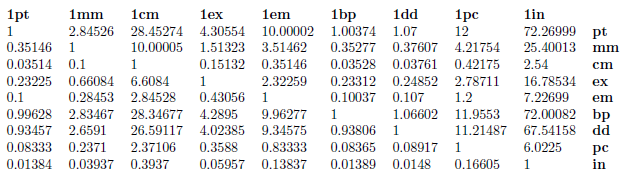
\includegraphics[scale=0.7]{measures.png}
    \caption{Unità di misura ammissibili in \LaTeX}
\end{figure}

\begin{giotikzpicture}
\draw (0,0) -- (0,1);
\end{giotikzpicture}

\begin{giotikzpicture}
\draw (0,0) -- (0,1cm);
\end{giotikzpicture}

\begin{giotikzpicture}
\draw (0,0) -- (0,5pt);
\end{giotikzpicture}

\subsubsection{Esercizio}
Disegnare due linee concentriche e ortogonali, lunghe 3cm.
\input{es-assi}

\subsection{Esempi di Move-to, Line-to}

\begin{giotikzpicture}
\draw (0,0) -- (1,1) (1,0) -- (2,1);
\end{giotikzpicture}

\begin{giotikzpicture}
\draw (0,0) -- (1,1)
      (1,0) -- (2,1);
\end{giotikzpicture}

\begin{giotikzpicture}
\draw (0,0) -- (1,1);
\draw (1,0) -- (2,1);
\end{giotikzpicture}

\begin{giotikzpicture}
\draw (-10,0) -- (-9,1) (0,0) -- (1,1) -- (1,0) -- (0,0);
\end{giotikzpicture}

\begin{giotikzpicture} % nota: non genera un path chiuso (come invece fa cycle). Zoomando nel documento si apprezza la differenza nei due casi.
\draw (-10,0) -- (-9,1) (0,0) -- (1,1) -- (1,0) -- (current subpath start);
\end{giotikzpicture}

\begin{giotikzpicture}
\draw (-10,0) -- (-9,1) (0,0) -- (1,1) -- (1,0) -- cycle;
\end{giotikzpicture}

\subsubsection{Esercizio}
Disegnare un quadrato di lato $1cm$.
\input{es-quadrato}

\subsection{Coordinate polari\riferimento{https://tikz.dev/tikz-coordinates}}
\begin{giotikzpicture}
\draw (0,0) -- (120:3);
\end{giotikzpicture}

\begin{giotikzpicture}
\draw (0,0) -- (120:3) -- (180:3) -- cycle;
\end{giotikzpicture}

\subsection{Movimento relativo (+ e ++)\riferimento{https://tikz.dev/tikz-coordinates\#sec-13.4}}

\begin{giotikzpicture}
\draw (10,0) -- +(120:3) -- +(180:3) -- cycle;
\end{giotikzpicture}

\begin{giotikzpicture}
\draw (10,0) -- ++(120:3) -- ++(180:3) -- cycle;
\end{giotikzpicture}

\begin{giotikzpicture}
\draw (10,0) -- ++(1,0);
\end{giotikzpicture}

\begin{giotikzpicture}
\draw (10,0) -- +(1,0);
\end{giotikzpicture}

\begin{giotikzpicture}
\draw (10,0) -- ++(1,0) -- +(0,1);
% oppure
% \draw (10,0) -- ++(1,0) -- ++(0,1);
\end{giotikzpicture}

\begin{giotikzpicture}
\draw (10,0) -- +(1,0) -- +(0,1);
% oppure
% \draw (10,0) -- +(1,0) -- ++(0,1);
\end{giotikzpicture}

\begin{giotikzpicture}
\draw (10,0) -- ++(1,0) -- (0,1);
% oppure:
% \draw (10,0) -- +(1,0) -- (0,1);
\end{giotikzpicture}

\subsubsection{Esercizio}
Una scaletta con scalini alti 0.2cm e lunghi 1cm.
\input{es-scaletta}

\subsubsection{Esercizio}
Disegnare un esagono di lato $1.2cm$.
\input{es-esagono}

\subsection{Opzioni\riferimento{https://tikz.dev/tikz-actions\#sec-15.3}}

\begin{giotikzpicture}
\draw[color=red] (1,0) -- ++(1,1);
\draw    [color=blue!20,line width=0.2pt] (2,0) -- ++(1,1);
% 
\draw[line width=0.2pt] (3,0) -- ++(1,1);
\draw[line width=0.1pt] (4,0) -- ++(1,1);
% 
\draw[red] (5,0) -- ++(1,1);
\draw[thin] (6,0) -- ++(1,1);
\draw[thick] (7,0) -- ++(1,1);
\draw[very thick] (8,0) -- ++(1,1);
\end{giotikzpicture}

\begin{giotikzpicture}[color=blue] % opzione globale
\draw[dashed] (1,0) -- ++(1,1);
\draw[dash dot] (2,0) -- ++(1,1);
\draw[densely dash dot dot] (3,0) -- ++(1,1);
\end{giotikzpicture}
\noindent Si possono cambiare le opzioni mentre si disegna:
% 
\begin{giotikzpicture}
\draw (0,0) -- (1,1)
       [rounded corners] -- (2,0) -- (3,1)
       [sharp corners] -- (3,0) -- (2,1);
\end{giotikzpicture}

\begin{giotikzpicture}
\draw (0,0) -- (1,1)
    {[rounded corners] -- (2,0) -- (3,1)}
    -- (3,0) -- (2,1);
\end{giotikzpicture}
\noindent Nota: ci sono alcune eccezioni. Ad esempio, il colore non si può cambiare mentre si disegna un path:

\begin{giotikzpicture}
\draw[yellow] (0,0) -- (1,1)
    {[rounded corners,black] -- (2,0) -- (3,1)}
    -- (3,0) -- (2,1);
\end{giotikzpicture}


\subsection{Frecce\riferimento{https://tikz.dev/tikz-arrows}}

\begin{giotikzpicture}
\draw[->,color=red] (1,0) -- ++(1,1);
\draw[<->,color=red] (2,0) -- ++(1,1);
\draw[>->,color=red] (3,0) -- ++(1,1) -- ++(1,1);
% necessitano della libreria arrows.meta
\draw[>-Stealth,color=red] (4,0) -- ++(1,1);
\draw[-{Stealth[red]}] (5,0) -- ++(1,1);
\draw[>-Latex] (6,0) -- ++(1,1);
\end{giotikzpicture}

\begin{giotikzpicture}[<->,scale=2,color=blue] % opzioni globali
\draw (0,0) -- ++(0,1);
\draw[opacity=0.3, dashed] (1,0) -- ++(0,1);
\end{giotikzpicture}

\newpage

\subsubsection{Esercizio}
Considerando l'esagono di prima, renderlo spesso $0.5cm$ e tratteggiato come in figura:
\input{es-esagono-grosso}

\subsubsection{Esercizio}
Raffigurare la regola del parallelogramma:
\input{es-parallelogramma}

\subsection{Coordinate nominate}

Rendo dinamica l'immagine usando le macro:

\newcommand{\veca}{0.5,0.7}
\newcommand{\vecb}{1.0,0.3}
\begin{giotikzpicture}
\draw[->] (0,0) -- (1.5,0);
\draw[->] (0,0) -- (0,1.5);
\draw[-Stealth,blue] (0,0) -- ++(\veca);
\draw[-Stealth,red] (0,0) -- ++(\vecb);
\draw[-Stealth,red] (\veca) -- +(\vecb);
\draw[-Stealth,blue] (\vecb) -- +(\veca);
\end{giotikzpicture}

\noindent Principale vantaggio: posso accedere alle macro anche qui:
{\em ``Regola del parallelogramma applicata ai vettori (\veca) e (\vecb)''}.

\noindent Principale svantaggio: ho limiti ``sconvenienti'' sui nomi da assegnare alle coordinate.

Alternativa: definisco una coordinata tramite il comando \texttt{\textbackslash coordinate}.

\begin{giotikzpicture}
\coordinate (vec1) at (0.5,0.7);
\coordinate (vec2) at (1.0,0.3);

\draw[->] (0,0) -- (1.5,0);
\draw[->] (0,0) -- (0,1.5);
\draw[-Stealth,blue] (0,0) -- ++(vec1);
\draw[-Stealth,red] (0,0) -- ++(vec2);
\draw[-Stealth,red] (vec1) -- +(vec2);
\draw[-Stealth,blue] (vec2) -- +(vec1);
\end{giotikzpicture}

\noindent Principale vantaggio: più leggibile e ``appropriato''.

\noindent Principale svantaggio: non posso riferire alla coordinata fuori dalla \texttt{tikzpicture}.

Le coordinate nominate aprono a un mondo di possibilità. Ad esempio, con la semplice opzione \texttt{label}\riferimento{https://tikz.dev/tikz-shapes\#sec-17.10.2} possiamo mostrare il nome di un punto del piano:

\begin{giotikzpicture}
\coordinate[label = v1] (vec1) at (0.5,0.7);
\coordinate[label = below:v2] (vec2) at (1.0,0.3);
% \coordinate[label = v2, position = below] (vec2) at (1.0,0.3); % Alternativa

\draw[->] (0,0) -- (1.5,0);
\draw[->] (0,0) -- (0,1.5);
\draw[-Stealth,blue] (0,0) -- ++(vec1);
\draw[-Stealth,red] (0,0) -- ++(vec2);
\draw[-Stealth,red] (vec1) -- +(vec2);
\draw[-Stealth,blue] (vec2) -- +(vec1);
\end{giotikzpicture}

\subsection{Coordinate calcolate\riferimento{https://tikz.dev/tikz-coordinates\#sec-13.5}}


Senza librerie esterne, Si possono fare alcuni semplici calcoli nel specificare le coordinate:

\begin{giotikzpicture}
\draw (0,0) -- ++(1+0,0+1);
\end{giotikzpicture}

\begin{giotikzpicture}
\coordinate (coord) at (1+0,0+1);
\draw (0,0) -- ++(coord);
\end{giotikzpicture}
\noindent Ma sono limitato, e a volte \TikZ\ non mi avverte dei suoi limiti.
% \begin{giotikzpicture}
% \draw (0,0) -- (2*(1,1)); % Questo potrebbe dare errore.
% % \draw (0,0) -- ++(2*(1,1)); % Questo dà errore
% \end{giotikzpicture}
% \noindent
Tramite la libreria \texttt{calc}, posso indicare a \TikZ\ come calcolare le coordinate in modi più complessi:
\begin{giotikzpicture}
\draw (0,0) -- ($2*(1,1)$);
\draw (0,0) -- ++($2*(1,1)$); % Nota: questo ora funziona
\end{giotikzpicture}
\noindent Si ricordino i \$, perché se mancano \TikZ\ potrebbe sbagliare silenziosamente.
% \begin{giotikzpicture}
% % 
% \draw (0,0) -- ++($0.5*(1,1)$);
% \draw (1,0) -- ++($(1,1)+(1,1)$);
% % 
% \draw (5,0) -- ++(0.5*(1,1));
% \draw (6,0) -- ++((1,1)+(1,1));
% % 
% \end{giotikzpicture}
I calcoli possono essere complessi. Esempio:
\begin{giotikzpicture}
\draw (0,0) --
     ($(0,0)+(1,0)$) --
     ($(0,0)+(1,0)+(0,1)$) --
     ($(0,0)+2*(1,0)+(0,1)$) --
     ($(0,0)+2*(1,0)+2*(0,1)$);
\end{giotikzpicture}

\subsubsection{Path-comando \texttt{coordinate}}

\begin{giotikzpicture}
\draw (0,0) coordinate[label=A](A) -- 
     ($(0,0)+(1,0)$) coordinate[label=B](B);
\end{giotikzpicture}

\subsubsection{Esercizio}

Provare a usare il path-comando \texttt{coordinate} per rendere dinamico il path rosso:
\begin{giotikzpicture}
\draw (0,0) -- 
     ($(0,0)+(1,0)$) --
     ($(0,0)+(1,0)+(0,1)$) --
     ($(0,0)+2*(1,0)+(0,1)$) --
     ($(0,0)+2*(1,0)+2*(0,1)$);
\draw[red] (0,0) -- ($(0,0)+(1,0)+(0,1)$) -- ($(0,0)+2*(1,0)+2*(0,1)$);
\end{giotikzpicture}

\input{es-coordinate}

\subsubsection{Alcuni calcoli interessanti: partway, distance, projection modifiers\riferimento{https://tikz.dev/tikz-coordinates\#sec-13.5}}

Sintassi comune: \textcolor{red}{prima coordinata}!\textcolor{blue}{modificatore}!\textcolor{red}{seconda coordinata}. A seconda della natura del modificatore, si interpreta questa operazione in maniera diversa.

\smallskip

\paragraph{Partway modifier\riferimento{https://tikz.dev/tikz-coordinates\#sec-13.5.3}} una {\em media pesata} tra due coordinate.
\begin{giotikzpicture}
\coordinate[label = A] (A) at (1,0);
\coordinate[label = B] (B) at (3,2);
\draw (A) -- (B);
\coordinate[label = C] (C) at ($(A)!0.75!(B)$);
\end{giotikzpicture}

\subsubsection{Esercizio}
Date due coordinate, e la linea che le congiunge, progettare un ciclo \texttt{\textbackslash foreach} che produca delle frecce; il risultato deve essere una serie di frecce che indichino i punti a 0\%, 20\%, 40\%, ..., lungo la linea, proseguendo fino a ricoprire il doppo della distanza tra le due coordinate:

\input{es-foreach0}

\paragraph{Distance modifier\riferimento{https://tikz.dev/tikz-coordinates\#sec-13.5.4}} movimento relativo rispetto al primo punto, in direzione di un secondo punto.

\begin{giotikzpicture}
\coordinate[label = A] (A) at (1,0);
\coordinate[label = B] (B) at (3,2);
\draw (A) -- (B);
\foreach \i in {1cm, 2cm, 3cm, -0.5cm}{
    \draw[<-,green] ($(A)!\i!(B)$) -- ++(-1,1);
}
\end{giotikzpicture}

\paragraph{Projection modifier\riferimento{https://tikz.dev/tikz-coordinates\#sec-13.5.5}} proiezione di un terzo punto lungo la linea che congiunge i due punti di riferimento.
\begin{giotikzpicture}
\coordinate[label = A] (A) at (1,0);
\coordinate[label = B] (B) at (3,2);
\coordinate[label = C] (C) at (-1,3);
\draw (A) -- (B);
\draw[<-,green] ($(A)!(C)!(B)$) -- ++(-1,1);

\end{giotikzpicture}

\newpage

\subsection{Linee verticali/orizzontali\riferimento{https://tikz.dev/tikz-paths\#sec-14.2.2}, Curve-To\riferimento{https://tikz.dev/tikz-paths\#sec-14.3}, archi\riferimento{https://tikz.dev/tikz-paths\#sec-14.7}}

\begin{giotikzpicture}
\draw (0,0) -- (1,1);
\draw (2,0) |- +(1,1);
\end{giotikzpicture}

\begin{giotikzpicture}
\draw[color=red] (0,0) .. controls (1,1) .. (4,0);
\draw[color=gray] (0,0) -- (1,1) -- (4,0);
\end{giotikzpicture}

\begin{giotikzpicture}
\draw[color=red] (0,0) .. controls (1,0) and (1,1) .. (0,1);
\draw[color=gray] (0,0) -- (1,0) -- (1,1) -- (0,1);
\end{giotikzpicture}

\begin{giotikzpicture}
  \draw[red] (0,0) arc[start angle = 30, end angle = 60, radius = 2cm];
  % \draw[red] (0,0) arc (30:60:2cm);
  \draw[gray] (0,0) -- ++(30+180:2cm) -- +(60:2cm);
\end{giotikzpicture}

\subsubsection{Esercizio}
Disegnare degli assi lunghi $1.5cm$ come in figura, ma usando una sola draw e il comando $|-$:

\input{es-assi2}

\subsection{Coordinate all'intersezione a linee perpendicolari\riferimento{https://tikz.dev/tikz-coordinates\#sec-13.3}}

\begin{giotikzpicture}
\draw[<->] (0,5) |- (5,0);
\draw[->,color=red] (2,1) -- (2,1 |- 3,4) -- (3,4);
\end{giotikzpicture}

\begin{giotikzpicture}
\draw[<->] (0,5) |- (5,0);
\coordinate (A) at (2,1);
\coordinate (B) at (3,4);
\draw[->,color=black,line width=.1cm] (A) |- (B);
\draw[->,color=white,line width=.03cm] (A) -- (A |- B) -- (B);
\end{giotikzpicture}

\noindent Utile per disegnare le proiezioni di un punto:
\begin{giotikzpicture}[gridded]
\coordinate[label = $A$] (A) at (30:3);
\draw[<->] (0,3.5) |- (3.5,0);
\draw[color=blue,text=black,dashed] (A) -- (A -| 0,0) coordinate[label=left:$f(x)$](B);
\draw[color=red,text=black,dashed] (A) -- (A |- 0,0) coordinate[label=below:$x$](C);
\draw[color=gray,text=black] (0,0) -- (A) circle (2pt);
\end{giotikzpicture}

\noindent È anche possibile calcolare le coordinate a intersezioni tra path complessi\riferimento{https://tikz.dev/tikz-coordinates\#sec-13.3.2}.

\subsection{Rettangoli\riferimento{https://tikz.dev/tikz-paths\#sec-14.4}, cerchi, ellissi\riferimento{https://tikz.dev/tikz-paths\#sec-14.6}}

\begin{giotikzpicture}
\draw[red] (0,0) rectangle (1,1);
\draw (.5,1) rectangle (2,0.5) -- (3,0) rectangle ++(.5,1.5) -- (5,0);
\end{giotikzpicture}

\begin{giotikzpicture}
\draw (1,0) circle; % non funziona perché il `radius` non è specificato
\draw (2,0) circle [radius=1]
    -- (4,0)
    circle [x radius=1cm, y radius=5mm]
    -- (6,0)
    ellipse [x radius=1cm, y radius=5mm, rotate=30];
\end{giotikzpicture}

\begin{giotikzpicture}[radius=2pt] % Uso una opzione globale, che viene propagata a tutti i comandi draw
\draw (1,0) circle;
\draw (2,0) circle;
\draw (3,0) circle;
\draw (4,0) circle;
\end{giotikzpicture}

\noindent Nota: anche \texttt{draw} ha una opzione \texttt{rotate}\riferimento{https://tikz.dev/tikz-transformations\#pgf.rotate}, diversa dalla \texttt{rotate} di \texttt{circle}; la prima ruota il tracciato attorno all'origine, la seconda disegna il cerchio già ruotato attorno al proprio centro:

% rotate around={60:(A)}
% https://tikz.dev/tikz-transformations

\begin{giotikzpicture}
\draw[<->] (0,1.5) |- (1.5,0);
\draw (1,0) circle [x radius=1cm, y radius=5mm, rotate=30] -- (2,0);
\end{giotikzpicture}

\begin{giotikzpicture}
\draw[<->] (0,1.5) |- (1.5,0);
\draw[rotate=60] (1,0) circle [x radius=1cm, y radius=5mm] -- (2,0);
\end{giotikzpicture}


\subsection{Comando \texttt{\textbackslash path}: bordi e riempimenti\riferimento{https://tikz.dev/tikz-actions}}

\texttt{\textbackslash path} è il principale comando \TikZ\ per disegnare tracciati.
A differenza di \texttt{\textbackslash draw}, di default, questo comando crea il tracciato ma non disegna nulla:

\begin{giotikzpicture}[gridded]
\path (0,0) circle (.5cm);
\path[red] (2,0) circle (.5cm);
\path[color=red] (4,0) circle (.5cm);
\draw[color=red] (6,0) circle (.5cm);
\draw[color=red,fill] (8,0) circle (.5cm);
\end{giotikzpicture}

\noindent Per disegnare il path, bisogna specificare l'opzione \texttt{draw}:
\begin{giotikzpicture}[gridded]
\path[draw] (0,0) circle (.5cm);
\path[draw,red] (2,0) circle (.5cm);
\path[draw,color=red] (4,0) circle (.5cm);
\draw[color=red] (6,0) circle (.5cm);
\draw[color=red,fill] (8,0) circle (.5cm);
\end{giotikzpicture}

\noindent In realtà, il comando \texttt{\textbackslash draw}, così come altri comandi è una istanza di \texttt{\textbackslash path}:

\begin{itemize}
\item \texttt{\textbackslash draw} = \texttt{\textbackslash path[draw]};
\item \texttt{\textbackslash fill} = \texttt{\textbackslash path[fill]};
\item \texttt{\textbackslash filldraw} = \texttt{\textbackslash path[fill,draw]};
\item ...
\end{itemize}

\begin{giotikzpicture}[gridded]
\path (0,0) circle (.5cm);
\draw (2,0) circle (.5cm);
\fill (4,0) circle (.5cm);
\filldraw (6,0) circle (.5cm);
\end{giotikzpicture}

\begin{giotikzpicture}[gridded]
\path (0,0) circle (.5cm);
\path[draw] (2,0) circle (.5cm);
\path[fill] (4,0) circle (.5cm);
\path[fill,draw] (6,0) circle (.5cm);
\end{giotikzpicture}

\noindent Di default, il colore specificato con \texttt{color} viene usato sia per il riempimento che per il bordo del tracciato:

\begin{giotikzpicture}[gridded, background grid/.style={draw,step=.5cm,very thin}]
\draw[color=red] (0,0) circle (.5cm);
\fill[color=red] (2,0) circle (.5cm);
\filldraw[color=red] (4,0) circle (.5cm);
\end{giotikzpicture}

\noindent Nota: il colore può anche essere passato direttamente come opzione (e.g., \texttt{thin}), senza specificare \texttt{color=}:

\begin{giotikzpicture}[gridded, background grid/.style={draw,step=.5cm,very thin}]
\draw[red] (0,0) circle (.5cm);
\fill[red] (2,0) circle (.5cm);
\filldraw[red] (4,0) circle (.5cm);
\end{giotikzpicture}

\noindent Tuttavia, si possono usare colori diversi per fill, draw:

\begin{giotikzpicture}[gridded, background grid/.style={draw,step=.5cm,very thin}]
\path[draw,red] (0,0) circle (.5cm);
\path[draw=blue,fill=red] (2,0) circle (.5cm);
\path[draw,blue,fill=red] (4,0) circle (.5cm);
\path[draw,color=blue,fill=red] (6,0) circle (.5cm);
\end{giotikzpicture}

\noindent A proposito, si possono controllare indipendentemente i colori per fill, draw, e per il testo generato nella costruzione path. Quando si specifica un colore come chiave (e.g., \texttt{[red]}) o tramite color (e.g., \texttt{[color=red]}), vengono settati automaticamente le tre chiavi:

\begin{itemize}
\item \texttt{fill color};
\item \texttt{draw color};
\item \texttt{text color}.
\end{itemize}

\begin{giotikzpicture}[gridded, background grid/.style={draw,step=.5cm,very thin}]
\path[draw,red] (0,0) circle (.5cm) coordinate[label=\textbf{C}];
\path[draw,fill,red] (2,0) circle (.5cm) coordinate[label=\textbf{C}];
\path[draw=blue,fill=red!20,text=yellow] (4,0) circle (.5cm) coordinate[label=\textbf{C}];
\path[draw,blue,fill=red!20] (6,0) circle (.5cm) coordinate[label=\textbf{C}];
\path[draw,color=blue,fill=red!20] (8,0) circle (.5cm) coordinate[label=\textbf{C}];
\end{giotikzpicture}

\noindent Un discorso simile può essere fatto per la chiave \texttt{opacity}, che controlla insieme \texttt{fill opacity}, \texttt{draw opacity} e \texttt{text opacity}.

\subsubsection{Riempimento con \texttt{fill}\riferimento{https://tikz.dev/tikz-actions\#sec-15.5}, \texttt{pattern}\riferimento{https://tikz.dev/tikz-actions\#sec-15.5.1}, \texttt{shade}\riferimento{https://tikz.dev/tikz-actions\#sec-15.7}}

La chiave \texttt{fill} controlla il riempimento dell'interno del path.

\begin{giotikzpicture}[gridded]
\path[draw=red,very thick,fill] (0,0) coordinate[label=left:$a$](a) -- (2,0) coordinate[label=$b$](b) -- (0,2) coordinate[label=$c$](c);
\end{giotikzpicture}

\begin{giotikzpicture}[gridded]
\path[draw=red,fill=green!20] (0,0) -- (2,0) -- (0,2) -- (0,-2) -- (-2,0) -- cycle;
\end{giotikzpicture}

\noindent Ma cos'è... l'interno? Dipende dalla \texttt{fill rule}\riferimento{https://tikz.dev/tikz-actions\#sec-15.5.2}:

\begin{giotikzpicture}[gridded]
\path[draw=red,fill=green!20] (0,0) -- ++(-1,1) -- ++(+2,+1) -- ++(+1,-1.5) -- ++(-2.0,0.5) -- ++(+2.0,0.5) -- cycle;
\path[draw=red,fill=green!20,nonzero rule] (4,0) -- ++(-1,1) -- ++(+2,+1) -- ++(+1,-1.5) -- ++(-2.0,0.5) -- ++(+2.0,0.5) -- cycle;
\path[draw=red,fill=green!20,even odd rule] (8,0) -- ++(-1,1) -- ++(+2,+1) -- ++(+1,-1.5) -- ++(-2.0,0.5) -- ++(+2.0,0.5) -- cycle;
\end{giotikzpicture}

\begin{giotikzpicture}[gridded]
\path[draw=red,fill=green!20] (0,0) circle (.5cm)  (0.5,0) circle (.5cm);
\path[draw=red,fill=green!20,even odd rule] (2,0) circle (.5cm)  (2.5,0) circle (.5cm);
\path[draw=red,fill=green!20,even odd rule] (4,0) circle (.5cm)  (4.5,0) circle (.5cm) (4.25,.5) circle (.5cm);
\path[draw=red,fill=green!20] (6,0) -- +(1,1) -- +(2,0) circle (.5cm);
\end{giotikzpicture}

% Altro riferimento utile: https://texnical-designs.com/fill-rules-in-tikz/

\noindent Esempio di fill con arco di circonferenza:
\begin{giotikzpicture}[gridded]
\path[fill=green!20] (0,0) arc[start angle = -90, end angle= 180, radius = 1cm];
\path[draw=red,fill=green!20, opacity=0.5] (2,0) arc[start angle = -90, end angle= 180, radius = 1cm];
\filldraw[red,fill=none, opacity=0.5] (4,0) arc[start angle = -90, end angle= 180, radius = 1cm];
\end{giotikzpicture}

\noindent Nota: la presenza di oggetti diversi da linee può influenzare il significato del riempimento.
\begin{giotikzpicture}
\draw[thick,fill=blue] (.5,1) rectangle (2,0.5) -- (3,0) rectangle ++(.5,1.5) -- (5,0);
\end{giotikzpicture}

\begin{giotikzpicture}
\draw[thick,fill=red] (.5,1) -- (2,0.5) -- (3,0) -- ++(.5,1.5) -- (5,0);
\end{giotikzpicture}

\noindent Riempimento con \texttt{pattern}\riferimento{https://tikz.dev/tikz-actions\#sec-15.5.1}\riferimento{https://tikz.dev/library-patterns}:

\begin{giotikzpicture}[gridded]
  \pattern[pattern color=black,pattern=bricks] (0,0) -- +(0,1) arc (180:0:1.5cm) -- +(0,-1);
\end{giotikzpicture}

\begin{giotikzpicture}[gridded]
  \def\mypath{(0,0) -- +(0,1) arc (180:0:1.5cm) -- +(0,-1)}
  \fill   [red]                                \mypath;
  \pattern[pattern color=white,pattern=bricks] \mypath;
\end{giotikzpicture}

% \begin{giotikzpicture}[gridded]
%     \coordinate[label=below:$a$] (a) at (1,1);
%     \fill[text=green!20] (a) arc[start angle = 180, end angle= 90, radius = 1cm] coordinate[label=right:$c$] (c);
%     % \fill[green!20] (a) arc[start angle = 180, end angle= 90, radius = 1cm] coordinate[label=right:$c$] (c);
%     \path[fill=green!20, opacity=0.5] (c) arc[start angle = -90, end angle= 180, radius = 1cm];
% \end{giotikzpicture}

\noindent Riempimento con \texttt{shade}\riferimento{https://tikz.dev/tikz-actions\#sec-15.7}:

\begin{giotikzpicture}[gridded]
\shadedraw[shading=axis] (0,0) rectangle +(1,1);
\shadedraw[shading=radial] (2,0) rectangle +(1,1);
\shadedraw[shading=ball] (4,0.5) circle (.5cm);
\shadedraw[shading=ball] (6.2,0) -- ++(60:1) -- ++(120:1) -- ++(180:1) -- ++(240:1) -- ++(300:1) -- cycle;
\end{giotikzpicture}

\begin{giotikzpicture}[gridded]
\shade[left color=red,right color=blue] (0,0) rectangle +(2,2);
\shade[top color=red,bottom color=blue] (4,0) rectangle +(2,2);
\end{giotikzpicture}

% \subsubsection{\texttt{clip}}

\subsubsection{Esercizio}

Disegnare questa girandola tramite comandi \texttt{\textbackslash filldraw} e \texttt{\textbackslash pattern}:

\input{es-girandola}

% Approfondimento: clipping https://tikz.dev/tikz-actions#sec-15.9

\subsection{Un po' di programmazione!}

\subsubsection{Ciclare con \texttt{\textbackslash foreach}\riferimento{https://tikz.dev/pgffor\#section-foreach}}

Disegno 4 ellissi ruotando sistematicamente ciascuno di essi:
\begin{giotikzpicture}
\foreach \i in {1,2,3,4}{
\draw (0,0) circle [rotate = 45*\i, x radius = 0.5cm, y radius = 2cm];
}
\end{giotikzpicture}


\noindent Può essere usato anche per generare path-comandi (e.g., dentro una \texttt{\textbackslash draw}):
\begin{giotikzpicture}
\draw (0,0)
\foreach \i in {1,2,3,4}{
circle [rotate = 45*\i, x radius = 0.5cm, y radius = 2cm]
};
\end{giotikzpicture}

% Notare i punto e virgola!

\begin{giotikzpicture}
\draw (0,0) \foreach \i in {(0,1),(1,0),(1,1)} {
-- \i
};
\end{giotikzpicture}

\subsubsection{Esercizio}
Disegnare 30 ellissi equicentrati, ruotati in modo da distribuirsi uniformemente:

\input{es-ellissi}

\subsubsection{Esercizio}
Trovare una soluzione all'esercizio precedente, generalizzata a $n$ ellissi:

\input{es-ellissi2}

\newpage
\subsubsection{Esercizio}

Riprendiamo la nostra scaletta con scalini alti 0.2cm e lunghi 1cm:
\begin{giotikzpicture}
\draw (0,0)
    -- ++(1,0) -- ++(0,.2)
    -- ++(1,0) -- ++(0,.2)
    -- ++(1,0);
\end{giotikzpicture}

\noindent E rendiamola parametrica nel numero di scalini, con uno dei due modi di ciclare, numerando ciascun scalino.

\input{es-scaletta2}


\noindent Posso indicare a \texttt{\textbackslash foreach} di salvarmi in una macro contatore il numero dell'iterazione (\texttt{count}):

\begin{giotikzpicture}
\newcommand{\tantiellissi}[1]{
\foreach \i [count=\xi from -4] in {1,...,#1}{
\fill[draw,fill=red,fill opacity=\i/#1] (0,0) circle [rotate = 360/2/#1*\i, x radius = 0.5cm, y radius = 2cm];
\coordinate[label=\xi] (c\xi) at (360/2/#1*\i:2cm);
}
}
\tantiellissi{9}
\end{giotikzpicture}

\subsubsection{Esercizio}

Nella figura precedente, è stata variata la \texttt{fill opacity}, che controlla la trasparenza/opacità del riempimento. Cambiare il codice della figura precedente in modo che, anzichè l'opacità, sia il colore stesso del riempimento a variare, e che questo vari tra rosso e bianco. Ricordiamo la sintassi per mischiare i colori: \texttt{\textit{colore1}!\textit{valorepercentuale}!\textit{colore2}}.

\input{es-ellissi3}

\noindent Possiamo usare la variabile del \textcomando{foreach} per creare coordinate in maniera sistemica:
\begin{giotikzpicture}
\draw \foreach \i in {1,2,...,10} {
\foreach \j in {1,2,...,3} {
(\i,\j) coordinate[label={\i,\j}](c\i-\j) circle[radius = 2pt]
}
};
% 
\filldraw[purple,fill opacity=0.2] (c1-1) -- (c2-3) -- (c3-2) -- cycle;
\end{giotikzpicture}

Tecniche avanzate per il \textcomando{foreach}:
\begin{itemize}
    % \item opzione \texttt{count-from} per contare le iterazioni;
    \item \texttt{Dot notation} nel specificare le liste:
    \begin{bloccoesempio}
        \foreach \x in {2^1,2^...,2^7} {$\x$, }
    \end{bloccoesempio}
    \begin{bloccoesempio}
        \foreach \x in {A_1,..._1,H_1} {$\x$, }
    \end{bloccoesempio}
    \item Opzione \texttt{evaluate-as-using} per assegnare a una macro una valutazione matematica sulla variabile:
    \begin{bloccoesempio}
        \foreach \x [evaluate=\x as \xvalutata] in {2^0,2^...,2^8}{$\x=\xvalutata$, }
    \end{bloccoesempio}
    \item Opzione \texttt{parse=true} per valutare matematicamente il limite superiore della lista di iterazione:
    \begin{bloccoesempio}
        \newcommand{\N}{10}
        \foreach \x [parse=true,evaluate=\x as \x] in {1/\N, 2/\N,...,1-1/\N}{$\x$, }
        \pgfmathsetmacro{\limitesuperiore}{1-1/\N}\limitesuperiore
    \end{bloccoesempio}
    \item Comando \textcomando{breakforeach} per terminare l'iterazione (utile se associato ai {\em condizionali}).
\end{itemize}

\subsubsection{Condizionali}

\begin{itemize}
    \item 

\texttt{\textbackslash ifnum} si può usare per verificare relazioni di uguaglianza, minoranza o maggioranza (=, <, >) tra numeri {\em interi}.
%
\begin{bloccoesempio}
\ifnum 5 < 6 YES \fi
\end{bloccoesempio}

\begin{bloccoesempio}
\ifnum -6 > 2 YES \else NO \fi
\end{bloccoesempio}

\begin{bloccoesempio}
\ifnum 2 = 2 YES \else NO \fi
\end{bloccoesempio}

% \ifnum \N > 20 \textcolor{red}{Attenzione! il numero di ellissi è troppo alto!} \fi

\item

\texttt{\textbackslash ifdim} è l'equivalente che funziona per numeri {\em reali}. È pensato per dimensioni \LaTeX, pertanto si aspetta unità di misura.

\begin{bloccoesempio}
\ifdim 4.3 pt < 4.1 pt YES \fi
\end{bloccoesempio}

\begin{bloccoesempio}
\ifdim 5.8 pt = 5.8 pt YES \else NO \fi
\end{bloccoesempio}

\item

\texttt{\textbackslash ifodd} testa la parità di un numero intero:
% 
\begin{bloccoesempio}
5 è un numero \ifodd 5 dispari\else pari\fi.
\end{bloccoesempio}

\item
Per confronti tra stringhe (i.e., sequenze di caratteri), consiglio il pacchetto \texttt{xifthen}, che mette a disposizione \texttt{\textbackslash ifthenelse}, unito a:
\begin{itemize}
\item \texttt{\textbackslash equal\{{\em str1}\}\{{\em str2}\}}: controlla l'uguaglianza tra stringhe;
\item \texttt{\textbackslash isempty\{{\em str}\}}: controlla se una stringa è vuota;
\item \texttt{\textbackslash isin\{{\em str1}\}\{{\em str2}\}}: controlla se una stringa appare come sottostringa di un'altra;
\item \texttt{\textbackslash endswith\{{\em str1}\}\{{\em str2}\}}: controlla che una stringa sia suffissata da un'altra.
\end{itemize}

\begin{bloccoesempio}
\ifthenelse{\equal{ciao}{ciao}}{TRUE}{FALSE}
\ifthenelse{\equal{ciao}{ciao2}}{TRUE}{FALSE}
\end{bloccoesempio}

\begin{bloccoesempio}
\newcommand{\checkciao}[1]{\ifthenelse{\equal{ciao}{#1}}{TRUE}{FALSE}}%
\checkciao{ciao}
\checkciao{ciao2}
\end{bloccoesempio}

\begin{bloccoesempio}
\ifthenelse{\isin{ia}{ciao}}{TRUE}{FALSE}
\ifthenelse{\endswith{ti dico ciao}{ciao}}{TRUE}{FALSE}
\end{bloccoesempio}
\end{itemize}

\noindent Naturalmente, la potenza dei condizionali sta nel fatto di poter espandere macro nelle condizioni:

\begin{bloccoesempio}
\newcommand{\ilmionumero}{5}
Il mio numero è \textbf{%
\ifodd \ilmionumero dis\fi pari} e
\textbf{\ifdim \ilmionumero cm > 4.2 cm maggiore \else minore \fi} di 4.2.
\end{bloccoesempio}

\medskip

\subsubsection{Esercizio live!}
Ho definito tre comandi \textcomando{equalitycheck},
\textcomando{minorecheck}, \textcomando{maggiorecheck} che confrontano due interi. Come li espando per accettare anche valori reali?

\begin{bloccoesempio}
\newcommand{\disparicheck}[1]{\ifodd #1YES\else NO\fi}
\newcommand{\equalitycheck}[2]{\ifnum #1=#2YES\else NO\fi}
\newcommand{\minorecheck}[2]{\ifdim #1 cm < #2 cm YES\else NO\fi}
\newcommand{\maggiorecheck}[2]{\ifnum #1>#2YES\else NO\fi}

\noindent \texttt{\textbackslash disparicheck}:
\disparicheck{4}
\disparicheck{5}
\\
\texttt{\textbackslash equalitycheck}:
\equalitycheck{5}{4}
\equalitycheck{4}{4}
\\
\texttt{\textbackslash maggiorecheck}:
\maggiorecheck{5}{4}
\maggiorecheck{4}{5}
\\
\texttt{\textbackslash minorecheck}:
\minorecheck{5}{4}
\minorecheck{4}{0}
\end{bloccoesempio}

\subsubsection{Esempio}
Condizionali innestati che controllano il colore:
\begin{giotikzpicture}
\foreach \i in {0, 0.3, ..., 3.0} {
\filldraw[line width = 0.2cm, fill opacity=0.4,
    \ifdim \i pt > 1.0 pt%
        \ifdim \i pt > 2.0 pt%
            purple%
        \else%
            blue%
        \fi%
    \else%
        red%
    \fi] (\i*3, 0) circle (0.45);
}
\end{giotikzpicture}

\subsubsection{Esercizio}
Disegnare una griglia $10\times 10$ di righe verticali e orizzontali,
con righe di spessore alternato \texttt{very thin}/\texttt{very thick}:

\input{es-griglia}

\subsubsection{Esercizio}

Disegnare una matrice di $12\times 12$ cerchi di raggio 10pt, riempiendo quelli sulla diagonale di rosso (o usando un \texttt{ball shading}):

\input{es-cerchi}

\subsubsection{Calcoli\riferimento{https://tikz.dev/math-parsing}}

\begin{itemize}
    \item 

\texttt{\textbackslash pgfmathparse} e \texttt{\textbackslash pgfmathresult} si possono usare per calcoli aritmetici generici:

\begin{bloccoesempio}%
\pgfmathparse{cos(60)*4.5}%
\pgfmathresult % Espande al valore dell'ultima \pgfmathparse
\let\w\pgfmathresult % lo assegno a una macro
%
\ifdim \pgfmathresult cm < 2 cm YES \else NO \fi
\end{bloccoesempio}

\begin{bloccoesempio}%
\pgfmathparse{5*2 > 10.1}%
\ifnum \pgfmathresult = 1 5*2 > 10.1 è vero\else 5*2 > 10.1 non è vero\fi
\end{bloccoesempio}

    \item 

\texttt{\textbackslash pgfmathsetmacro} e \texttt{\textbackslash pgfmathtruncatemacro} assegnano il valore calcolato da una espressione aritmetica ad una macro specificata (similmente a \textcomando{newcommand}).
\\\texttt{\textbackslash pgfmathsetmacro} si usa per calcoli tra numeri {\em reali},
\\\texttt{\textbackslash pgfmathtruncatemacro} tronca il risultato, e si usa tra numeri {\em interi}.

\begin{bloccoesempio}
\pgfmathsetmacro\ilmiovalore{sqrt(abs(cos(120)*4.5))}
\ilmiovalore
\end{bloccoesempio}

\begin{bloccoesempio}
\pgfmathtruncatemacro\ilmiovalore{sqrt(abs(cos(120)*4.5))}
\ilmiovalore
\end{bloccoesempio}

\begin{bloccoesempio}
\pgfmathsetmacro\ilmiovalore{int(sqrt(abs(cos(120)*4.5)))}
\ilmiovalore
\end{bloccoesempio}


\end{itemize}

\subsubsection{Esercizio}

Cambiare la politica di riempimento della matrice di prima, riempiendo i cerchi che stanno sulla parabola
\[y=\left[\frac{x^2}{10}\right]:\]

\input{es-cerchi-parabola}

 
\subsection{Esercizio}

Creare un comando \texttt{\textbackslash girandola}, che disegni $n$ quadrati strutturati nella seguente maniera:

\input{es-quadraticerchi}

\newpage


\subsection{Nodi\riferimento{https://tikz.dev/tikz-shapes}}

Un nodo si comporta come una coordinata, ma ha una {\em estensione}, una {\em forma} e un {\em contenuto}.
Similmente alle coordinate, si crea con il comando \textcomando{node}, o con il path-comando \texttt{node} dentro un \textcomando{path}; il {\em contenuto} viene specificato in coda al comando, dentro a graffe:

\begin{giotikzpicture}
\coordinate (coord0) at (-2,0); % Non disegna nulla
\node (nodo0) at (-2,0) {N0};
% specifico una forma a cerchio
\node[circle] (nodo1) at (-1,0) {N1};
\node[circle, text=red, fill = blue!20, draw = blue, ultra thick] (nodo2) at (0,0) {N2};
% Un nodo è molto diverso da una coordinata con etichetta!
\coordinate[label={C0}] (C0) at (1,0);
\coordinate[label={[label distance=0cm]C1}] (C1) at (2,0);
% Nota: segnalo la posizione delle coordinate
\draw[fill = blue!20, draw = blue, ultra thick]
    (C0) circle (2pt)
    (C1) circle (2pt);
\end{giotikzpicture}
% 
\noindent Si noti la differenza tra nodo con testo e coordinata con etichetta. L'etichetta è sempre apposta a lato della coordinata, anche quando si specifica una distanza nulla.
% 
In realtà, la coordinata è un tipo particolare di nodo, senza forma né contenuto:
\begin{center}\texttt{\textcomando{coordinate[{\em \color{red} opzioni}]} {\em ...}} $\equiv$ \texttt{\textcomando{node[coordinate,{\em \color{red} opzioni}]} {\em ...} \{\}};\end{center}
% 
La forma di un nodo si può specificare tramite l'opzione \texttt{shape} (oppure anche elidendo l'assegnazione \texttt{shape=}). Di default, sono disponibili le forme {\em circle}, {\em rectangle}, e, appunto, {\em coordinate}:
\begin{giotikzpicture}
\node[shape=circle] at (-2,0) {N0}; % Notare che (come per le coordinate) posso non dare un nome al nodo
\node[circle,red] at (-1,0) {N1};
\node[circle,draw=red] at (0,0) {N1};
\node[circle, fill = blue!20, draw = blue, ultra thick] at (1,0) {N2};
\node[rectangle, fill = blue!20, draw = blue, rounded corners=1pt, ultra thick] at (2,0) {N3};
\node[rectangle] at (3,0) {N4};
\node[coordinate, fill = blue!20, draw = blue, ultra thick] at (4,0) {N5}; % Notare che non viene mostrata
\end{giotikzpicture}
% 
\newpage\noindent Altre forme per i nodi (e.g., diamante, ellisse, trapezio, ...) sono disponibili nella libreria \texttt{shapes}\riferimento{https://tikz.dev/library-shapes\#section-libs-shapes}.
% 
\begin{giotikzpicture}
\foreach \shappp [count=\j] in {
    coordinate,
    rectangle,
    circle,
    diamond,
     trapezium,
    ellipse callout,
    cloud,
    forbidden sign,
    starburst} {
\node[draw,\shappp,fill=blue!30] at (0,-2*\j) {\shappp};
}
\end{giotikzpicture}


\newpage
Per esempio: \texttt{regular polygon}:
\begin{giotikzpicture}
\newcommand{\poligonoregolare}[5][]{%
\node [#1,
    draw,
    shape=regular polygon,
    regular polygon sides=#3,
    minimum size=#4*#3
] (#5) at #2 {};%
}
\foreach \i [count=\numerolati from 3] in {-4,...,3}{
\poligonoregolare[rounded corners=0.7pt, violet, fill=cyan]{(\i,0)}{\numerolati}{0.1cm}{poly\i}
}
\draw[red] (poly-4) -- 
(poly-3) -- 
(poly-2) -- 
(poly-1) -- 
(poly0) -- 
(poly1) -- 
(poly2) -- 
(poly3);
\end{giotikzpicture}


Uno dei punti forti dei nodi sta nelle {\em line shortening rules}, che permettono di trattare il nodo come un {\em oggetto geometrico} dotato di una area interna ed una esterna. Il suo uso risulta, di conseguenza, sostanzialmente diverso rispetto a quello delle coordinate; per esempio, un path che collega nodi con estensione (ovvero nodi che non sono coordinate) non può essere riempito:
\begin{giotikzpicture}[every node/.style={draw}]
\path
(0,0) coordinate(b1)
(1,0) coordinate(b2)
(1,1) coordinate(b3)
(0,1) coordinate(b4);
\filldraw[fill=yellow!80!black] (b1) -- (b2) -- (b3) -- (b4);

\path[xshift=1.5cm,shape=rectangle,fill=blue] % Note: fill does not work!
(0,0) node(a1){}
(1,0) node(a2){}
(1,1) node(a3){}
(0,1) node(a4){};
\filldraw[fill=yellow!80!black] (a1) -- (a2) -- (a3) -- (a4);
\end{giotikzpicture}

\newpage
\subsubsection{Geometria del nodo\riferimento{https://tikz.dev/tikz-shapes\#sec-17.2.3}}

La struttura geometrica di un nodo può essere semplificata così:
% 
\input{es-nodegeom}

\noindent
Partendo dall'interno:
\begin{itemize}
\item La dimensione del contenuto viene gestita in automatico;
\item I padding (o {\em spaziature interne}) si posson specificare con {\em {\bfseries inner} sep}/{\em xsep}/{\em ysep};
\item La dimensione del bordo si può specificare con {\em line width};
\item I margini (o {\em spaziature esterne}) si posson specificare con {\em {\bfseries outer} sep}/{\em xsep}/{\em ysep};
\end{itemize}
Inoltre, la {\em dimensione minima} dell'area di filling (contenuto+padding) si posson specificare con {\em {\bfseries minimum} size}/{\em width}/{\em height}.
Di default, un nodo ha un poco di spaziatura interna, ma spaziatura esterna nulla.
% Notare uso di opzioni globali e dell'opzione "every node/.style"!
\begin{giotikzpicture}[
    xscale=2.0,
    every path/.style={thick,-Latex},
    every node/.style={
        rectangle,
        text = white,
        fill = red!50,
        draw = black
    }
]
% Controllo padding con inner sep/xsep/ysep
\node[] (N0) at (0,0) {\hl{N0}};
\node[inner sep=0pt] (N1) at (1,0) {\hl{N1}};
\node[inner xsep=0.4cm, inner ysep=0.2cm] (N2) at (2,0) {\hl{N2}};
\draw (N0) -- (N1);
\draw (N1) -- (N2);
% Controllo margin con outer sep/xsep/ysep
\node[outer sep=0pt] (N3) at (0,-1) {\hl{N3}};
\node[outer sep=0.2cm] (N4) at (1,-1) {\hl{N4}};
\node[outer xsep=-5pt] (N5) at (2,-1) {\hl{N5}};
\draw (N3) -- (N4);
\draw (N4) -- (N5);
% Controllo area di filling con minimum size/width/height
\node[minimum size=1cm] (N6) at (0,-2) {\hl{N6}};
\node[minimum width=1cm, minimum height=0.5cm] (N7) at (1,-2) {\hl{N7}};
\node[minimum width=1cm] (N8) at (2,-2) {\hl{N8}};
\draw (N6) -- (N7);
\draw (N7) -- (N8);
\end{giotikzpicture}
% 
\noindent Si noti la l'uso di \texttt{every path/.style} e \texttt{every node/.style}, che permette l'assegnazione di opzioni a tutti i nodi o tutti i path all'interno di una \texttt{tikzpicture}\riferimento{https://tikz.dev/tikz-shapes\#tikz/every:node}.

Cogliamo l'occasione per presentare le opzioni per controllare lo scaling della figura: \texttt{scale}/\texttt{xscale}/\texttt{yscale}.
Queste riscalano lo spazio di disegno, ricalcolando le coordinate dei nodi prima di disegnarli, ma lasciando le dimensioni dei nodi invariate.
La stessa figura senza \texttt{xscale=2.0} si presenta come:
\begin{giotikzpicture}[
    every path/.style={thick,-Latex},
    every node/.style={
        rectangle,
        text = white,
        fill = red!50,
        draw = black
    }
]
% Controllo padding con inner sep/xsep/ysep
\node[] (N0) at (0,0) {\hl{N0}};
\node[inner sep=0pt] (N1) at (1,0) {\hl{N1}};
\node[inner xsep=0.4cm, inner ysep=0.2cm] (N2) at (2,0) {\hl{N2}};
\draw (N0) -- (N1);
\draw (N1) -- (N2);
% Controllo margin con outer sep/xsep/ysep
\node[outer sep=0pt] (N3) at (0,-1) {\hl{N3}};
\node[outer sep=0.2cm] (N4) at (1,-1) {\hl{N4}};
\node[outer xsep=-5pt] (N5) at (2,-1) {\hl{N5}};
\draw (N3) -- (N4);
\draw (N4) -- (N5);
% Controllo area di filling con minimum size/width/height
\node[minimum size=1cm] (N6) at (0,-2) {\hl{N6}};
\node[minimum width=1cm, minimum height=0.5cm] (N7) at (1,-2) {\hl{N7}};
\node[minimum width=1cm] (N8) at (2,-2) {\hl{N8}};
\draw (N6) -- (N7);
\draw (N7) -- (N8);
\end{giotikzpicture}
% 
\noindent La stessa figura con \texttt{scale=2.0} si presenta come:
\begin{giotikzpicture}[
    scale=2.0,
    every path/.style={thick,-Latex},
    every node/.style={
        rectangle,
        text = white,
        fill = red!50,
        draw = black
    }
]
% Controllo padding con inner sep/xsep/ysep
\node[] (N0) at (0,0) {\hl{N0}};
\node[inner sep=0pt] (N1) at (1,0) {\hl{N1}};
\node[inner xsep=0.4cm, inner ysep=0.2cm] (N2) at (2,0) {\hl{N2}};
\draw (N0) -- (N1);
\draw (N1) -- (N2);
% Controllo margin con outer sep/xsep/ysep
\node[outer sep=0pt] (N3) at (0,-1) {\hl{N3}};
\node[outer sep=0.2cm] (N4) at (1,-1) {\hl{N4}};
\node[outer xsep=-5pt] (N5) at (2,-1) {\hl{N5}};
\draw (N3) -- (N4);
\draw (N4) -- (N5);
% Controllo area di filling con minimum size/width/height
\node[minimum size=1cm] (N6) at (0,-2) {\hl{N6}};
\node[minimum width=1cm, minimum height=0.5cm] (N7) at (1,-2) {\hl{N7}};
\node[minimum width=1cm] (N8) at (2,-2) {\hl{N8}};
\draw (N6) -- (N7);
\draw (N7) -- (N8);
\end{giotikzpicture}%
% 
\newpage
\noindent Invece, con \texttt{scale=5.0} e un \textcomando{resizebox} esterno l'immagine si presenta così:
\\
\begin{figure}[H]%
\centering%
\begin{framed}%
{\centering
\resizebox{0.75\textwidth}{!}{
\begin{tikzpicture}[
    scale=5.0,
    every path/.style={thick,-Latex},
    every node/.style={
        rectangle,
        text = white,
        fill = red!50,
        draw = black
    }
]
% Controllo padding con inner sep/xsep/ysep
\node[] (N0) at (0,0) {\hl{N0}};
\node[inner sep=0pt] (N1) at (1,0) {\hl{N1}};
\node[inner xsep=0.4cm, inner ysep=0.2cm] (N2) at (2,0) {\hl{N2}};
\draw (N0) -- (N1);
\draw (N1) -- (N2);
% Controllo margin con outer sep/xsep/ysep
\node[outer sep=0pt] (N3) at (0,-1) {\hl{N3}};
\node[outer sep=0.2cm] (N4) at (1,-1) {\hl{N4}};
\node[outer xsep=-5pt] (N5) at (2,-1) {\hl{N5}};
\draw (N3) -- (N4);
\draw (N4) -- (N5);
% Controllo area di filling con minimum size/width/height
\node[minimum size=1cm] (N6) at (0,-2) {\hl{N6}};
\node[minimum width=1cm, minimum height=0.5cm] (N7) at (1,-2) {\hl{N7}};
\node[minimum width=1cm] (N8) at (2,-2) {\hl{N8}};
\draw (N6) -- (N7);
\draw (N7) -- (N8);
\end{tikzpicture}
}
}
\end{framed}%
\end{figure}%

\newpage

\subsubsection{Posizionamento (in breve)\riferimento{https://tikz.dev/tikz-shapes\#sec-17.5}}

I {\em punti di ancoraggio} di un nodo sono utilizzati anche per fissare la posizione del nodo in una data coordinata.
\begin{figure}[H]
    \centering
    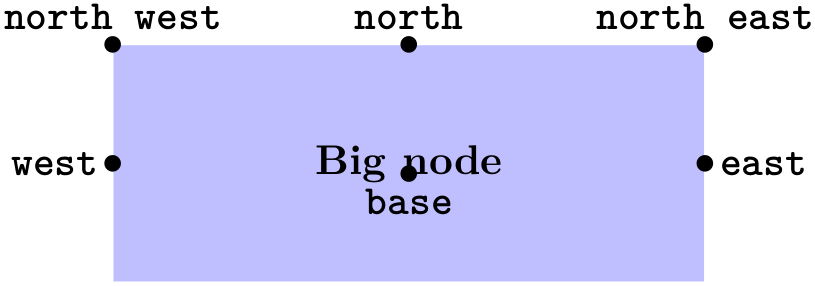
\includegraphics[scale=1.0]{anchors.png}
    % \caption{Punti di ancoraggio per un nodo \texttt{rectangle}}
    \label{fig:anchors}
\end{figure}

\noindent Di default, un nodo è ancorato al centro di una coordinata; altrimenti, si può specificare un punto di ancoraggio specifico tramite l'opzione {\em anchor}:
\begin{giotikzpicture}
\foreach \anch [count=\j] in {
    base,east,north east,north,north west,west,south west,south,south east} {
\node[draw,anchor=\anch,fill=blue!30,minimum size=.6cm] at (1.3*\j,0) {};
\filldraw (1.3*\j,0) circle (2pt);
}
\end{giotikzpicture}

\noindent ... Oppure tramite le opzioni di posizionamento {\em above}, {\em below}, {\em left}, {\em right} (e le opzioni combinate, e.g., {\em above right}):
\begin{giotikzpicture}
\foreach \posx [count=\j] in {
    above,
    below,
    left,
    right,
    above right,
    } {
\node[draw,\posx,fill=blue!30,minimum size=.6cm] (N\j) at (1.3*\j,0) {N\j};
\filldraw (1.3*\j,0) circle (2pt);
}
\end{giotikzpicture}

% \begin{giotikzpicture}[node distance=1cm]
% \node[draw,above,fill=blue!30,minimum size=.6cm] (N0) at (0,0) {N0};
% \filldraw (0,0) circle (2pt);
% \foreach \posx [count=\j] in {
%     right of =N0,
%     % right=2cm of N1, ???
%     above of=N3.north east
%     } {
% \node[draw,\posx,fill=blue!30,minimum size=.6cm] (N\j) at (1.3*\j,0) {N\j};
% \filldraw (1.3*\j,0) circle (2pt);
% }
% \end{giotikzpicture}

\newpage
\subsubsection{Archi\riferimento{https://tikz.dev/tikz-shapes\#sec-17.11}}

Una linea tra due nodi si chiama tipicamente {\em arco}.
In \TikZ, gli archi si possono disegnare con \textcomando{path}, usando le tipiche operazioni per linee dritte, curve, etc.
Come anticipato, gli archi uscenti da, e entranti in un certo nodo vengono disegnati non a partire dalla coordinata di posizione del nodo, ma dai {\bf punti di ancoraggio}:
% 
\begin{giotikzpicture}
% Notare l'uso degli scope. Ref: https://tikz.dev/tikz-scopes#sec-12.3
\begin{scope}
\node (x) at (0,0) {Nodo 1};
\node[draw] (y) at (3,1) {Nodo 2};
\draw[->,red]    (x) -| (y);
\draw[->,blue]   (x) -- (y);
\draw[->,orange] (x) .. controls +(up:1cm) and +(left:1cm) .. (y);
\end{scope}

\begin{scope}[yshift=-2.4cm]
\node[circle] (x) at (0,0) {Cerchio 1};
\node[circle,draw] (y) at (3,1) {Cerchio 2};
\draw[->,red]    (x) -| (y);
\draw[->,blue]   (x) -- (y);
\draw[->,orange] (x) .. controls +(up:1cm) and +(left:1cm) .. (y);
\end{scope}
\end{giotikzpicture}

\noindent Oltre ai path-comandi che già conosciamo, introduciamo il conveniente path-comando \texttt{to}\riferimento{https://tikz.dev/tikz-paths\#sec-14.13}. Funziona come una Line-to, ma permette di specificare curvature in maniera più elastica:
% 
\begin{giotikzpicture}
\node[circle,draw] (n1) at (0,0) {Nodo 1};
\node[circle,draw] (n2) at (2,0) {Nodo 2};
\node[circle,draw] (n3) at (4,0) {Nodo 3};
\node[circle,draw] (n4) at (8,0) {Nodo 4};
%

% Senza opzioni è equivalente a --, mentre con opzioni genera curve
\draw[->,red]    (n1) to (n2);
\draw[->,blue]   (n1) to[bend right] (n2);
\draw[->,orange] (n1) to[bend left] (n2);
% Curvatura con angoli di entrata e uscita dai nodi
\draw[->,red]    (n2) to (n3);
\draw[->,blue]   (n2) to[out=90] (n3);
\draw[->,orange] (n2) to[out=45,in=235] (n3);
% Scioltezza
\draw[->,red]    (n3) to[out=45,in=235,looseness=0.2] (n4);
\draw[->,blue]   (n3) to[out=45,in=235] (n4);
\draw[->,orange] (n3) to[out=45,in=235,looseness=3.0] (n4);
\end{giotikzpicture}
% 
\noindent Gestione particolare dei {\em loop}\riferimento{https://tikz.dev/library-edges\#tikz/loop}:
\begin{giotikzpicture}[thick,-Latex]
\node[circle,draw] (n1) at (0,0) {Nodo 1};
\node[circle,draw] (n2) at (3,0) {Nodo 2};
% Loop "sbagliato" vs gestione manuale
\draw[red] (n1) to (n1);
\draw[orange] (n1) to[out=-120,in=-30,looseness=2.8] (n1);
% Gestione automatica
\draw[black] (n2) to[loop] (n2);
\draw[orange] (n2) to[loop left] (n2);
\draw[red] (n2) to[loop above] (n2);
\draw[blue] (n2) to[loop below] (n2);
\end{giotikzpicture}

\noindent Una caratteristica interessante dei path-comandi è la possibilità di creare nodi {\em lungo} la linea disegnata:
% 
\begin{giotikzpicture}[thick,-Latex]
\draw[black] (0,0) to node {A} (3,2);
\draw[red] (0,0) to[out=90,in=180] node {B} (3,2);
\draw[blue!70] (0,0) to[out=110,in=90,looseness=2.0] node [pos=0.2] {C} (3,2);
\draw[orange] (0,0) to[out=-60,in=-90]
    node [pos=0.25] {25\%}
    node [pos=0.5] {50\%}
    node [pos=0.75] {75\%}
    node [pos=1.0] {100\%}
    (3,2);              
\end{giotikzpicture}

\noindent Si possono ottenere risultati eleganti controllando il posizionamento dei nodi. Per esempio, combinando le opzioni {\em sloped}, {\em above}, e {\em below}:
\begin{giotikzpicture}[thick,-Latex,every node/.style={sloped}]
\begin{scope}[above]
\draw[black] (0,0) to node {A} (3,2);
\draw[red] (0,0) to[out=90,in=180] node {B} (3,2);
\draw[blue!70] (0,0) to[out=110,in=90,looseness=2.0] node [pos=0.2] {C} (3,2);
\end{scope}
\begin{scope}[below]
\draw[orange] (0,0) to[out=-60,in=-90]
    node [pos=0.25] {25\%}
    node [pos=0.5] {50\%}
    node [pos=0.75] {75\%}
    node [pos=1.0] {100\%}
    (3,2);
\end{scope}
\end{giotikzpicture}

\noindent Più nodi su una linea possono essere creati sistematicamente con \texttt{node foreach}\riferimento{https://tikz.dev/tikz-shapes\#sec-17.8}:
\begin{giotikzpicture}[thick,-Latex]
\draw[black] (0,0) to (3,2);
% `node foreach` su una operazione `to`
\draw[blue!70] (0,0) to[out=90,in=90,looseness=2.0]
    node foreach \pos [count = \i] in {0.0,0.25,...,1}
        [
            draw,
            sloped,
            above,
            inner sep = 2pt,
            pos=\pos
        ] (x\i) {\pos}
     (3,2);
\begin{scope}[xshift=4cm]
\draw[black] (0,0) to (3,2);
% `node foreach` su una operazione `-|`
\draw[orange!70] (0,0) -|
    node foreach \pos [count = \i] in {0.0,0.25,...,1}
        [
            draw,
            sloped, % Nota: mostra anche con questo
            above,
            inner sep = 2pt,
            pos=\pos
        ] (x\i) {\pos}
     (3,2);
\end{scope}
\end{giotikzpicture}

\subsubsection{Accenni allo scoping, chiavi \texttt{every} e stili}

Come anticipato, l'environment \texttt{scope}\riferimento{https://tikz.dev/tikz-scopes\#sec-12.3} permette di limitare l'effetto di alcune opzioni a un blocco specifico di comandi. Questo è molto utile se utilizzato in coppia con chiavi come \texttt{every node/.style}, che permette di assegnare stili a tutti i nodi nello stesso scope dove viene applicato:

\begin{giotikzpicture}[
    every node/.style={draw=black,fill=black!20}
]
% Scope: tikzpicture esterna
\node (N1) at (0,0) {N1};
\node (N2) at (2,0) {N2};
\draw (N1) -- (N2);
\begin{scope}[
    yshift=-1cm,
    every node/.style={draw=red,fill=red!20},
    every path/.style={dashed,ultra thick,red}
]
% Scope: primo livello
\node (N1) at (0,0) {N1};
\node (N2) at (2,0) {N2};
\draw (N1) -- (N2);
\begin{scope}[
    yshift=-1cm,
    every node/.style={draw=blue,fill=blue!20},
    every path/.style={solid}
    % every path/.append style={solid}
]
% Scope: secondo livello
\node (N1) at (0,0) {N1};
\node (N2) at (2,0) {N2};
\draw (N1) -- (N2);
\end{scope}
\end{scope}
\end{giotikzpicture}

\noindent Si noti che, in realtà, gli scope limitano anche la visibilità esterna dei nodi definiti al loro interno (nella figura precedente \texttt{N1} e \texttt{N2} sono stati definiti più volte a diversi livelli).
% 
Simili a \texttt{every node} e \texttt{every path}, esistono anche
\texttt{every to} e
\texttt{every loop} e
\texttt{every scope} e
\texttt{every picture}.
% \begin{scope}[every node/.append style=mystyle]
%   \path (0,0) node(nodeThree) {Node Three} 
%       ++(5,0) node(nodeFour) {Node Four};
% \end{scope}

% every node/.style
% every node/.append style
% every path/.style={draw=...}
% every to/.style={bend left}
% every loop/.style={}

% every scope/.style={}
% % every picture/.append style

% \texttt{tikzset}...

Una funzionalità molto utile è quella di definire degli stili personalizzati.
Questo si può fare tramite \texttt{tikzstyle}\riferimento{https://tikz.dev/pgfkeys\#sec-87.4.4}, e gli stili possono anche essere parametrici, come in:
% 
{
\begin{minted}{latex}
\tikzstyle{my style}=[draw=red,fill=red!20]
\tikzstyle{my style}[red]=[draw=#1,fill=#1!20]
\end{minted}
}

{
\tikzstyle{my style}[red]=[draw=#1,fill=#1!20]
\begin{giotikzpicture}[my style2/.style={draw=#1,fill=#1!20}]
  \node [my style]  at (0,0)  {red box};
  \node [my style=blue] at (0,-1) {blue box};
  \node [my style2=blue] at (0,-2) {blue box$^2$};
\end{giotikzpicture}
}

\noindent Usando gli stili è possibile limitare ripetizioni e rindondanze nel codice, e si può rendere un codice \TikZ\ contemporaneamente più leggibile e facile da modificare.

\subsubsection{Esercizio}
Riprodurre il seguente diagramma:
\input{es-coinflipping}

\subsubsection{Esercizio}

Riprodurre il seguente diagramma:
\input{es-mobius}

Letture aggiuntive:
\begin{itemize}
\item Nodi di testo\riferimento{https://tikz.dev/tikz-shapes\#sec-17.4.3};
\item ~osizionamento auto e swap\riferimento{https://tikz.dev/tikz-shapes\#sec-17.8};
\item Grafi\riferimento{https://tikz.dev/tikz-graphs};
\item Grafi ad albero\riferimento{https://tikz.dev/tikz-trees}.
\end{itemize}

% edge operation

% letture aggiuntive:
% \begin{itemize}
% \item
    % Posizionamento e label:
    % spiegare il posizionamento: https://tikz.dev/tikz-shapes#sec-17.5
    % label position [label={[xshift=1em, yshift=-1em]
    % [label={[xshift=1em, yshift=-1em]}
% \item Pin https://tikz.dev/tikz-shapes#sec-17.10.3
% \item opzioni per controllare il testo
% \item puoi fare tanti nodi col foreach dentro:
% \begin{giotikzpicture}
% \node foreach \x in {1,...,4} foreach \y in {1,2,3}
%             [draw] at (\x,\y) {\x,\y};
% \end{giotikzpicture}
% \item tikzpicture dentro ad un nodo
% \item nodi multi-part, every lower node part
% \end{itemize}


% \tikzset{every picture/.append style={remember picture}}


% \begin{itemize}
%     \item remember picture+overlay per collegare due tikzpicture diverse
%   % \begin{tikzpicture}[remember picture]
%     % e poi: \draw[overlay] 
% \end{itemize}

% edge operation https://tikz.dev/tikz-shapes#sec-17.12


\subsubsection{Esercizio}

Riprodurre il diagramma che mostra la struttura di un nodo.
Sapendo che dentro ad un nodo può andare una \texttt{tikzpicture}!
Se si stilizza appropriatamente la geometria dei nodi, è possibile farlo usando tre o quattro nodi {\em innestati} in \texttt{tikzpicture}.

\subsubsection{Doppio bordo}

\begin{giotikzpicture}[every node/.style={rectangle,text = white, fill = red, draw = black},xscale=2.0] % Notare uso di opzioni globali e dell'opzione "every node/.style"!
\node[minimum size=1cm] (N6) at (0,-2) {\hl{N6}};
\node[minimum width=1cm,minimum height=0.5cm] (N7) at (1,-2) {\hl{N7}};
\node[minimum width=1cm] (N8) at (2,-2) {\hl{N8}};
\draw[->] (N6) -- (N7);
\draw[->] (N7) -- (N8);
% 
\begin{scope}[every node/.append style={draw,double=green,double distance=0.5mm}]
\node[minimum size=1cm] (N9) at (0,-3.2) {\hl{N9}};
\node[minimum width=1cm,minimum height=0.5cm] (N10) at (1,-3.2) {\hl{N10}};
\node[minimum width=1cm] (N11) at (2,-3.2) {\hl{N11}};
\draw[-{LaTeX},double distance=0.5mm, double=green] (N9) -- (N10);
\draw[-{LaTeX},double distance=0.5mm, double=green] (N10) -- (N11);
\end{scope}
\end{giotikzpicture}

% - double, double distance sia sul nodo che sulle draw.

\newpage



\subsection{Plot di funzione\riferimento{https://tikz.dev/tikz-plots}}

Il path-comando \texttt{plot} si usa per plottare funzioni. L'opzione \texttt{domain} controlla il dominio della varibile indipendente:

\begin{giotikzpicture}
\draw[blue] (0,0) circle (2pt) plot[domain = 1:2] (\x,2*\x);
\draw[red] plot[domain = 2:3] (\x,10-3*\x);
\draw[green] plot[domain = 3:6] (\x,0.06*\x^2);
\draw[domain = 6:8]
    plot (\x,0.3*\x)
    plot (\x,0.01*\x^2)
    plot (\x,0.001*\x^3);
\end{giotikzpicture}

\noindent Si possono usare funzioni del motore matematico (nota: quando si usano parentesi tonde, è meglio chiudere l'espressione in un gruppo con \{ e \} per preservare le parentesi tonde):

\begin{giotikzpicture}
% \draw[blue,domain = 0:1] plot (\x,sin(10*\x)); % Questo dà errore
% Meglio
\draw[red,domain = 1:2] plot (\x,{sin(10*\x)});
\end{giotikzpicture}

\noindent Per funzioni trigonometriche (e.g., \texttt{sin(\textbackslash x)}) la variabile viene interpretata in gradi sessaggesimali. Si può, però, indicare che l'angolo è da interpretare in radianti: \texttt{sin(\textbackslash x r)}.

\begin{giotikzpicture}
% Angolo in gradi
\draw[red,domain = 1:3,dashed] plot (\x,{sin(10*\x)});
% Angolo in radianti
\draw[blue,domain = 1:3,thick] plot (\x,{sin(10*\x r)});
\end{giotikzpicture}

\noindent Internamente, \texttt{plot} fa un certo numero di iterazioni per calcolare le coppie di coordinate, e poi esegue delle Line-to per unirle. Di default, vengono fatte 15 iterazioni equispaziate, ma questo a volte risulta troppo approssimativo; si può, allora, specificare un sampling più fine tramite l'opzione \texttt{samples}.

\begin{giotikzpicture}
% Sampling automatico (15)
\draw[red,domain = 1:5] plot (\x,{sin(10*\x r)});
% Sampling più fine
\draw[blue,domain = 5:10,samples=100] plot (\x,{sin(10*\x r)});
\end{giotikzpicture}

\noindent Sempre in ottica di ottenere \texttt{plot} meno spezzati, l'opzione \texttt{smooth} indica a draw di unire i samples non con spezzate ma con linee curve polinomiche. Attenzione, l'interpolazione curva può dare risultati inaspettati:

\begin{giotikzpicture}[mark=x,mark options={color=gray}]
% Sampling automatico (15)
\draw[red,domain = 1:2] plot (\x,{sin(10*\x r)});
% Sampling più fine
\draw[purple,domain = 2:4,samples=50] plot (\x,{sin(10*\x r)});
% Sampling smooth
\draw[blue,domain = 4:6,smooth] plot (\x,{sin(10*\x r)});
% Sampling smooth: problemi
\draw[green!70!black,domain = 6:8,smooth,samples=10] plot (\x,{sin(10*\x r)});
% % Sampling smooth: problemi
% \draw[red,domain = 8:10,smooth,samples=10,tension = 0.55] plot (\x,{sin(10*\x r)});
\end{giotikzpicture}

\noindent Come si vede nella precedente figura, è possibile aggiungere dei segni (o {\em mark}) in corrispondenza di ciascun sample del plot\riferimento{https://tikz.dev/tikz-plots\#sec-22.7}. Le opzioni per controllare lo stile dei segni sono: \texttt{mark}, \texttt{mark size}, \texttt{mark options}. Inoltre, si può limitare quali sample segnare con \texttt{mark repeat} e \texttt{mark phase} o, alternativamente, \texttt{mark indices}.

\begin{giotikzpicture}
\draw[red,domain = 1:2, mark=+] plot (\x,{sin(10*\x r)});
\draw[blue,domain = 2:4, mark=o, mark size=1pt] plot (\x,{sin(10*\x r)});
\draw[purple,domain = 4:6, mark=triangle*, mark options = {color=green, rotate=25, draw=black}] plot (\x,{sin(10*\x r)});
% Più fine
\begin{scope}[yshift=-2cm]
\draw[red,domain = 1:2, mark=+, mark repeat = 3] plot (\x,{sin(10*\x r)});
\draw[blue,domain = 2:4, mark=o, mark size=1pt, mark repeat = 3, mark phase = 3] plot (\x,{sin(10*\x r)});
\draw[purple,domain = 4:6, mark=triangle*, mark options = {color=green, rotate=25}, mark indices = {1,2,3,4,10,...,1000}] plot (\x,{sin(10*\x r)});
\end{scope}
% Più fine
\begin{scope}[samples=100,yshift=-4cm]
\draw[red,domain = 1:2, mark=+] plot (\x,{sin(10*\x r)});
\draw[blue,domain = 2:4, mark=o, mark size=1pt, mark repeat = 3, mark phase = 3] plot (\x,{sin(10*\x r)});
\draw[purple,domain = 4:6, mark=triangle*, mark options = {color=green, rotate=25}, mark indices = {1,2,3,4,10,...,1000}] plot (\x,{sin(10*\x r)});
\end{scope}
\end{giotikzpicture}

% \noindent Oltre a \texttt{+}, \texttt{o} e \texttt{triangle*}, altri tipi di marks sono disponibili con una volta importata la libreria \textcomando{plotmarks}.
\noindent Diversi tipi di marks sono disponibili con \textcomando{usetikzlibrary\{plotmarks\}}\riferimento{https://tikz.dev/library-plot-marks}.

Di default, la variabile indipendente è assegnata a \texttt{\textbackslash x}, ma il nome di questa macro si può controllare con l'opzione \texttt{variable}, per maggiore leggibilità. Questo è particolarmente utile quando si voglion plottare funzioni parametriche:

% \begin{giotikzpicture}
% \draw[red,domain=0:5,variable=\lamiavariabile] plot (\lamiavariabile,{0.2*(\lamiavariabile^2)});
% \draw[blue,domain=0:5,variable=\lamiavariabile] plot ({0.2*(\lamiavariabile^2)},\lamiavariabile);
% \draw[green!40!black,domain=0:1,variable=\lamiavariabile] plot (\lamiavariabile^2,\lamiavariabile^3);
% \end{giotikzpicture}

\begin{giotikzpicture}
\foreach \i/\colorr [count = \xsh] in {2/red,3/blue,5/green!50!black,7/black} {
\begin{scope}[xshift=2*\xsh cm]
\draw[\colorr,domain = -3.15:3.15,variable=\t,samples=200] plot ({sin(\i*\t r)},{cos(5*\t r});
% \draw[\colorr,domain = 0:360,variable=\ang,samples=200] plot (\ang:\i*\ang/200);
\end{scope}
}
\end{giotikzpicture}


\newpage
Oltre a \texttt{smooth}, esistono altri tipi di giunture tra samples\riferimento{https://tikz.dev/tikz-plots\#sec-22.8
}:
\begin{giotikzpicture}[
    domain=0:10,
    % Definisco la mia funzione, `giofun`.
    declare function = {
        giofun(\x)={0.3*sin(2*\x r)};
        giofun2(\x)={0.3*sin(2*\x r)};
    }
]
% Standard plot
\draw[yshift=-0cm] plot (\x,{giofun(\x)});
\draw[yshift=-1cm] plot[smooth] (\x,{giofun(\x)});
\draw[yshift=-2cm] plot[const plot] (\x,{giofun(\x)});
\draw[yshift=-3cm] plot[only marks,mark=*] (\x,{giofun(\x)});
% Plot costanti
\draw[yshift=-4cm] plot[const plot mark left,mark=*] (\x,{giofun(\x)});
\draw[yshift=-5cm] plot[const plot mark right,mark=*] (\x,{giofun(\x)});
\draw[yshift=-6cm] plot[jump mark left,mark=*] (\x,{giofun(\x)});
\draw[yshift=-7cm] plot[jump mark right,mark=*] (\x,{giofun(\x)});
% Altri
\draw[yshift=-8cm] plot[ycomb,mark=*] (\x,{giofun(\x)});
\draw[yshift=-9cm] plot[ybar,mark=*] (\x,{giofun(\x)});
% 
\foreach \ax in {0,1,...,10} {
\pgfmathsetmacro{\ay}{giofun(\ax)}
\coordinate[label=\ax] (C\ax) at (\ax,\ay);
}
\end{giotikzpicture}

\newpage
Come per altri path-comandi, alla fine di un \texttt{plot} si può costruire un \texttt{node} o una \texttt{coordinate} tramite i path-comandi appositi.

\begin{giotikzpicture}
\draw[very thin,color=gray] (-0.1,-1.1) grid (3.9,3.9);
\draw[->] (-0.2,0) -- (4.2,0) node[right] {$x$};
\draw[->] (0,-1.2) -- (0,4.2) node[above] {$f(x)$};
% 
\draw[red,jump mark right,domain=0:4]    plot (\x,\x)             node[right] {$f(x) =x$};
\draw[blue,mark=ball,domain=0:4]   plot (\x,{sin(\x r)})    node[right] {$f(x) = \sin x$};
\draw[orange,domain=0:4] plot (\x,{0.05*exp(\x)}) node[right] {$f(x) = \frac{1}{20} \mathrm e^x$};
% 
\coordinate[label=A] (A) at (2.5,2.5);
\draw[dashed,thick] (A) -- (A |- 0,0) node[below] {$x_1$};
\draw[dashed,thick] (A) -- (A -| 0,0) node[left] {$f(x_1)$};
\end{giotikzpicture}

\subsubsection{Esercizio}
Replicare il seguente plot della funzione $f(x) = 0.2x^3 - 2.4x$ per $x \in [-3,4]$, facendo uso di nodi ancorati (e.g., \texttt{node[left,...]}), \texttt{foreach}, e \texttt{declare function}:

\input{es-curva1}

\newpage
\subsubsection{Esercizio}
Replicare la curva
\begin{minted}{latex}
\draw (1, 1.7)
   .. controls (1.6, 2.4) .. (1.8, 2.4)
   .. controls (2.3, 2.4) and (2.4, 0.5) .. (3, 0.5)
   .. controls (3.5, 0.5) and (4.1, 3.1) .. (4.6, 3.1)
   .. controls (5, 3.1) and (5, 1.5) .. (5.4, 1.5)
   .. controls (5.6, 1.5) .. (6, 2.1);       
\end{minted}
come raffigurato nel seguente plot:
\input{es-curva2}

\subsubsection{Esercizio}
Replicare il seguente grafico raffigurante una distribuzione gaussiana:
\input{es-gaussiana}

% Il manuale di \TikZ\ fornisce strumenti specifici per Data Visualization\riferimento{https://tikz.dev/dv}.

\section{Ringraziamenti}
Ringrazio il Dr. Jonathan Franceschi, autore di parte del materiale da cui ho attinto nella stesura,
e il Prof. Damiano Foschi per l'aiuto nell'organizzazione del corso.

\end{document}

